\section{Durchführung}
\label{sec:Durchführung}
Der Aufbau des Versuchs ist in Abbildung \ref{fig:tfig3} dargestellt. 
Bei der verwendeten Probe handelt es sich um eine zu $0,005\%$ mit $\text{Sr}^{++}$-Atomen dotierte Kaliumbromidprobe.
Dieser Kristall ist hygroskopisch, er bindet also Feuchtigkeit aus der Umgebung.
Um dies zu verhindern wird der Rezipient vor dem Versuch bis zu einem Druck von $10^{-2}\,\text{mbar}$ evakuiert.

\begin{figure}[H]
    \begin{subfigure}{0.40\textwidth}
    \centering
    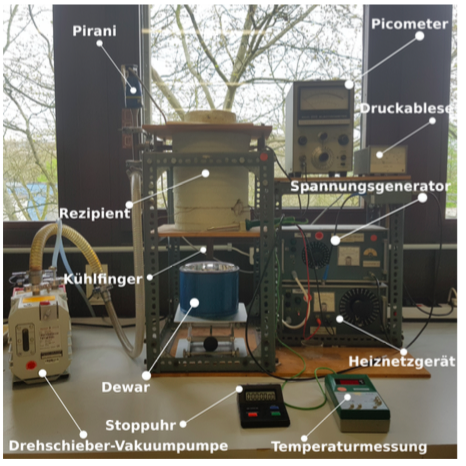
\includegraphics[width=\linewidth]{figs/aufbau}
    \end{subfigure}
    \begin{subfigure}{0.58\textwidth}
    \centering
    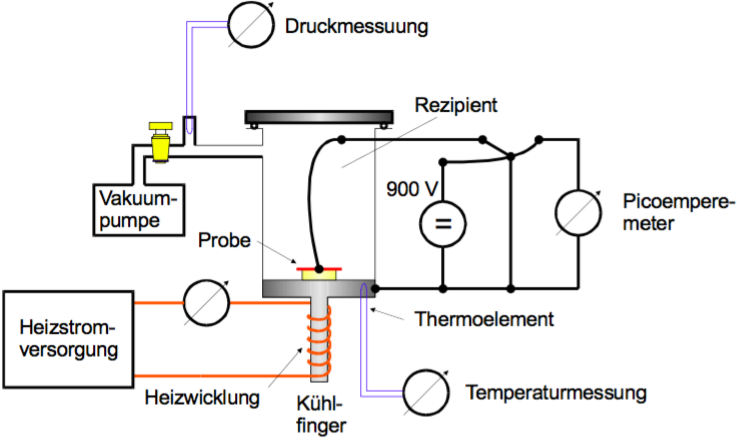
\includegraphics[width=1.1\linewidth]{figs/aufbau2}
    \end{subfigure}
    \caption{Photographische und schematische Darstellung des Versuchsaufbaus \cite{skript}.}
    \label{fig:tfig3}
\end{figure}

Zu Beginn wird die Probe durch Anlegen einer Heizspannung auf $\SI{320}{\K}$ erwärmt, sodass die 
Relaxationszeit möglichst klein wird.
Anschließend wird der Kondensator mit einer Spannung von $\SI{950}{\V}$ aufgeladen und $\SI{900}{\s}$ gewartet, bis eine stationäre Polarisation der Probe erzeugt wurde.
Durch das Eintauchen des Kühlfingers in flüssigen Stickstoff wird die Probe auf eine Temperatur von $\SI{210}{K}$ abgekühlt und der Polarisationszustand somit eingefroren.
Nachdem die Temperatur erreicht ist, wird das elektrische Feld abgeschaltet und der Kondensator für $\SI{5}{\min}$ kurzgeschlossen, damit alle beweglichen Ladungsteile in der Probe verschwinden und nur die Dipole verbleiben.

Um den Depolarisationsstrom zu messen wird das Picoamperemeter angeschlossen und der Strom so lange beobachtet, bis sich ein konstanter Wert eingestellt hat.
Daraufhin wird die Heizspannung erneut eingeschaltet, sodass sich eine konstante Heizrate von $\SI{2}{\K}$ pro Minute einstellt.
Während des Erwärmungsprozesses wird etwa alle $\SI{30}{\s}$ Temperatur und Depolarisationsstrom notiert, bis die Probe etwa eine Temperatur von $\SI{330}{\K}$ erreicht.

Zuletzt wird der gesamte Messvorgang für eine Heizrate von $\SI{1,5}{\K}$ pro Minute wiederholt.

